\documentclass[letterpaper]{article}
\usepackage[draft]{aaai2026}
\usepackage{times}
\usepackage{helvet}
\usepackage{courier}
\usepackage{iftex}
\ifPDFTeX
\usepackage[T1]{fontenc}
\else
\usepackage{fontspec}
\IfFileExists{/usr/share/fonts/urw-base35/NimbusRoman-Regular.otf}{%
\setmainfont{NimbusRoman}[Path=/usr/share/fonts/urw-base35/,Extension=.otf,UprightFont=*-Regular,BoldFont=*-Bold,ItalicFont=*-Italic,BoldItalicFont=*-BoldItalic]
\setsansfont{NimbusSans}[Path=/usr/share/fonts/urw-base35/,Extension=.otf,UprightFont=*-Regular,BoldFont=*-Bold,ItalicFont=*-Italic,BoldItalicFont=*-BoldItalic]
\setmonofont{NimbusMonoPS}[Path=/usr/share/fonts/urw-base35/,Extension=.otf,UprightFont=*-Regular,BoldFont=*-Bold,ItalicFont=*-Italic,BoldItalicFont=*-BoldItalic]
}{%
\setmainfont{TeX Gyre Termes}
\setsansfont{TeX Gyre Heros}
\setmonofont{TeX Gyre Cursor}
}
\fi
\usepackage[hyphens]{url}
\urlstyle{rm}
\def\UrlFont{\rm}
\usepackage{natbib}
\usepackage{caption}
\frenchspacing
\setlength{\pdfpagewidth}{8.5in}
\setlength{\pdfpageheight}{11in}
\ifPDFTeX
\pdfinfo{/TemplateVersion (2026.1)}
\fi
\setcounter{secnumdepth}{2}
\usepackage{graphicx}
\usepackage{tikz}
\usetikzlibrary{arrows.meta,positioning}
\usepackage{booktabs}
\usepackage{array}
\usepackage{amsmath}
\title{Regularization and Overfitting in DeBERTa-v3 on RTE}
\author{QIN HAOCHEN$^{1}$ \quad WANG YUMENG$^{2}$\\
YUAN ZHENGXI$^{3}$ \quad LING YUHE$^{4}$}
\affiliations{AI6128 Group 6, Nanyang Technological University\\
$^{1}$G2609647L \quad $^{2}$G2604731G \quad $^{3}$G2609829B \quad $^{4}$G2609682G}
\begin{document}
\maketitle

\begin{abstract}
We compare regularization methods for DeBERTa-v3-base on RTE using 12 epochs and seven seeds. Each method is compared with the same baseline. The Optimized Combination includes only methods that improve on the baseline under our four-of-seven rule. On the previously examined 374-example internal holdout, it reached 84.64\% mean accuracy versus 80.33\% for the baseline, a paired gain of 4.32 percentage points; all seven seeds improved. This comparison is exploratory, not an independent test.
\end{abstract}

\section{Question and Design}
We test regularization when fully fine-tuning DeBERTa-v3-base on GLUE's Recognizing Textual Entailment (RTE) task \cite{deberta,glue}. Each standalone method is compared with the same full-fine-tuning baseline. R-Drop adds a penalty when two dropout passes produce different predictions \cite{rdrop}.

RTE is part of GLUE, a widely used benchmark, and tests whether a hypothesis follows from a premise rather than whether the sentences share words. Its roughly 2.5k training examples make experiments inexpensive and easy to repeat across seeds. The two labels, ``entailment'' and ``not\_entailment'', make accuracy easy to interpret. RTE's small size also makes overfitting visible through a gap between training and development scores. The task has a long history in the PASCAL challenges, and its Hugging Face release supports reproducibility.

Every run uses 12 epochs and the same seven seeds: 123, 456, 789, 1011, 201765793, 1801564980, and 1323889826. Four existing seeds were retained and three randomly generated seeds were added. We use a learning rate of $3\times10^{-5}$, batch size 32, and weight decay 0.01. Candidate settings are selected by mean final development accuracy; lower development loss breaks ties. A method enters the Optimized Combination only if its mean paired gain is positive and at least four of seven seeds beat the baseline.

\subsection{Data Split and Preprocessing}
We divide the 2,490 labeled examples in the GLUE RTE training set into three grouped, label-stratified partitions. We group exact premise--hypothesis pairs before splitting so duplicates stay together.
\begin{table*}[tp]
\centering\small\setlength{\tabcolsep}{5pt}
\caption{RTE data used in this study. Percentages apply to the 2,490-example GLUE training split.}
\label{tab:data-splits}
\begin{tabular}{lrrp{0.52\textwidth}}
\toprule
Partition & Share & Examples & Use \\
\midrule
Training & 70\% & 1,742 & Fit models; generated examples, when used, are added to this split only \\
Development & 15\% & 374 & Select candidate settings and decide which methods enter the Optimized Combination \\
Internal holdout & 15\% & 374 & Compare the frozen baseline and Optimized Combination after selection \\
Official RTE validation & Separate & 277 & Not used in this comparison \\
\bottomrule
\end{tabular}
\end{table*}

We tokenize each premise--hypothesis pair with the DeBERTa-v3-base tokenizer and truncate sequences to 128 tokens. No additional text normalization is applied. For the held-out comparison, we retrain the baseline and the frozen Optimized Combination on the training split for each seed, then calculate accuracy on the 374-example internal holdout. We compare the two accuracies within each seed. Earlier project analyses also evaluated this split, so it was held out from fitting and selection in this study but is not an untouched test set.

\section{Six Regularization Techniques}
Regularization methods address different problems that can arise with small datasets. Recent work studies stable fine-tuning on low-resource text and regularization for generalization and calibration on GLUE \cite{somayajula2024,jukic2025}. Those papers study different methods; we cite them as context, not as evidence for our results. Each figure shows mean training and development loss over 12 epochs across seven seeds; the selected candidate is marked. We choose the candidate with the best mean final development accuracy; ties go to lower mean development loss, then the smaller setting. These choices are preliminary because they use the same development set for selection and evaluation.

\subsection{Filtered FLAN-T5 Augmentation}
FLAN-T5 generates alternative or lightly edited hypotheses from training premises \cite{flan}. A filter keeps a generated example only when the model predicts its intended label with confidence of at least 0.85. More examples can add useful variety, but generation may change meaning or introduce wrong labels. We compare requested ratios of 0.25, 0.50, and 1.00; the available filtered examples may limit the amount added. We augment training data only.
Figure~\ref{fig:curve-augmentation} compares all augmentation candidates with the baseline.
\IfFileExists{selection_results.tex}{%
\IfFileExists{curves_augmentation.pdf}{%
\begin{figure*}[tp]
\centering
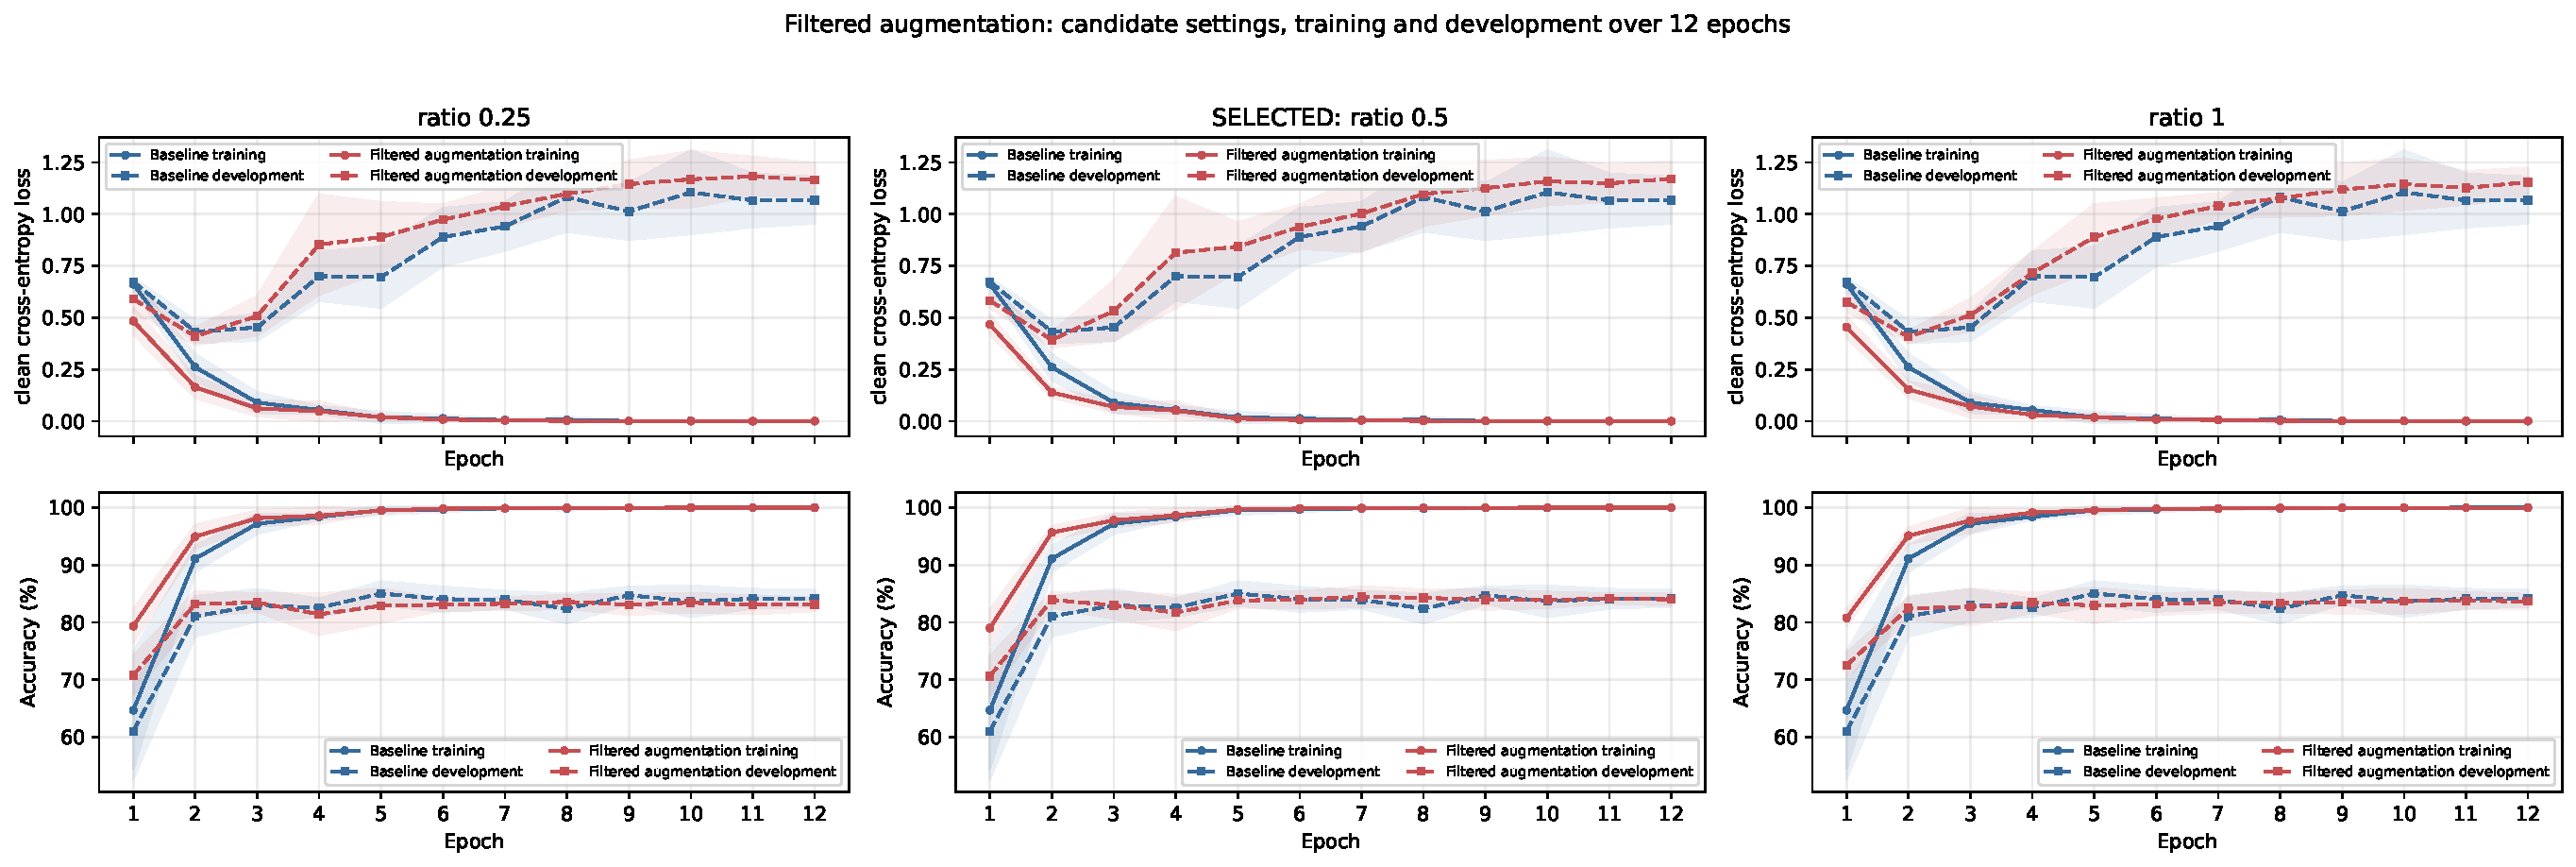
\includegraphics[width=0.96\textwidth]{curves_augmentation.pdf}
\caption{Loss and accuracy over 12 epochs for the three augmentation ratios. Lines show seven-seed means; shading shows $\pm1$ standard deviation. The selected ratio is marked.}
\label{fig:curve-augmentation}
\end{figure*}
}{}
}{}

\subsection{Label Smoothing}
With two classes, label smoothing replaces the one-hot target $y$ with $(1-\epsilon)y+\epsilon/K$ \cite{smoothing}. Softer targets may reduce overconfidence, but too much smoothing can blur class differences and cause underfitting. Kobyzev et al. also found that label regularization does not always help pretrained models \cite{kobyzev2023}. We compare $\epsilon\in\{0.05,0.10,0.15\}$.
Figure~\ref{fig:curve-label-smoothing} compares the three smoothing strengths with the baseline.
\IfFileExists{selection_results.tex}{%
\IfFileExists{curves_label_smoothing.pdf}{%
\begin{figure*}[tp]
\centering
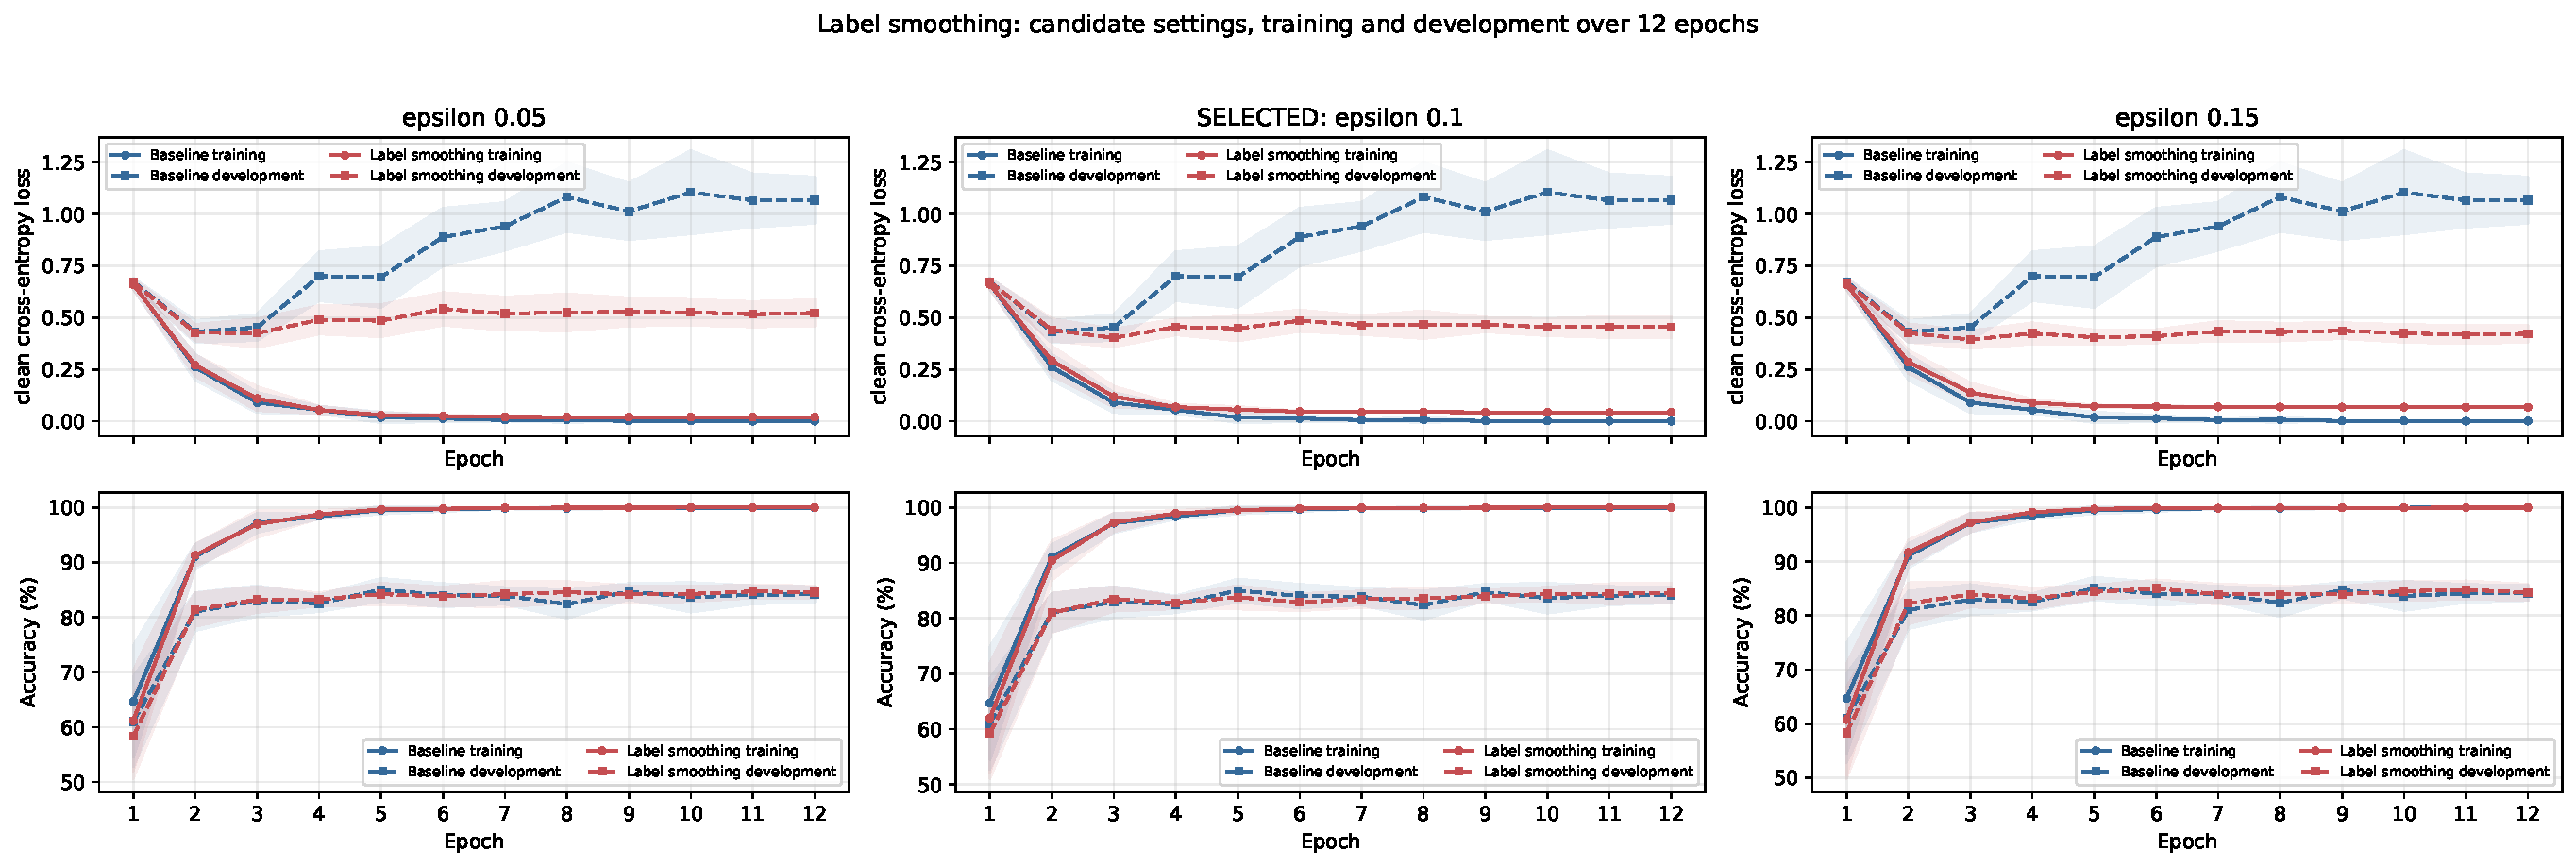
\includegraphics[width=0.96\textwidth]{curves_label_smoothing.pdf}
\caption{Loss and accuracy over 12 epochs for the three smoothing strengths. Lines show seven-seed means; shading shows $\pm1$ standard deviation. The selected value is marked.}
\label{fig:curve-label-smoothing}
\end{figure*}
}{}
}{}

\subsection{Embedding Mixup}
Mixup combines pairs of input embeddings and their labels using $\lambda\sim\operatorname{Beta}(\alpha,\alpha)$ \cite{mixup}. This can smooth predictions between examples and reduce memorization. Larger $\alpha$ means stronger mixing, but excessive mixing can obscure the entailment relation. We compare $\alpha\in\{0.1,0.2,0.4\}$. The attention mask includes tokens from both examples.
Figure~\ref{fig:curve-mixup} compares the three mixup strengths with the baseline.
\IfFileExists{selection_results.tex}{%
\IfFileExists{curves_mixup.pdf}{%
\begin{figure*}[tp]
\centering
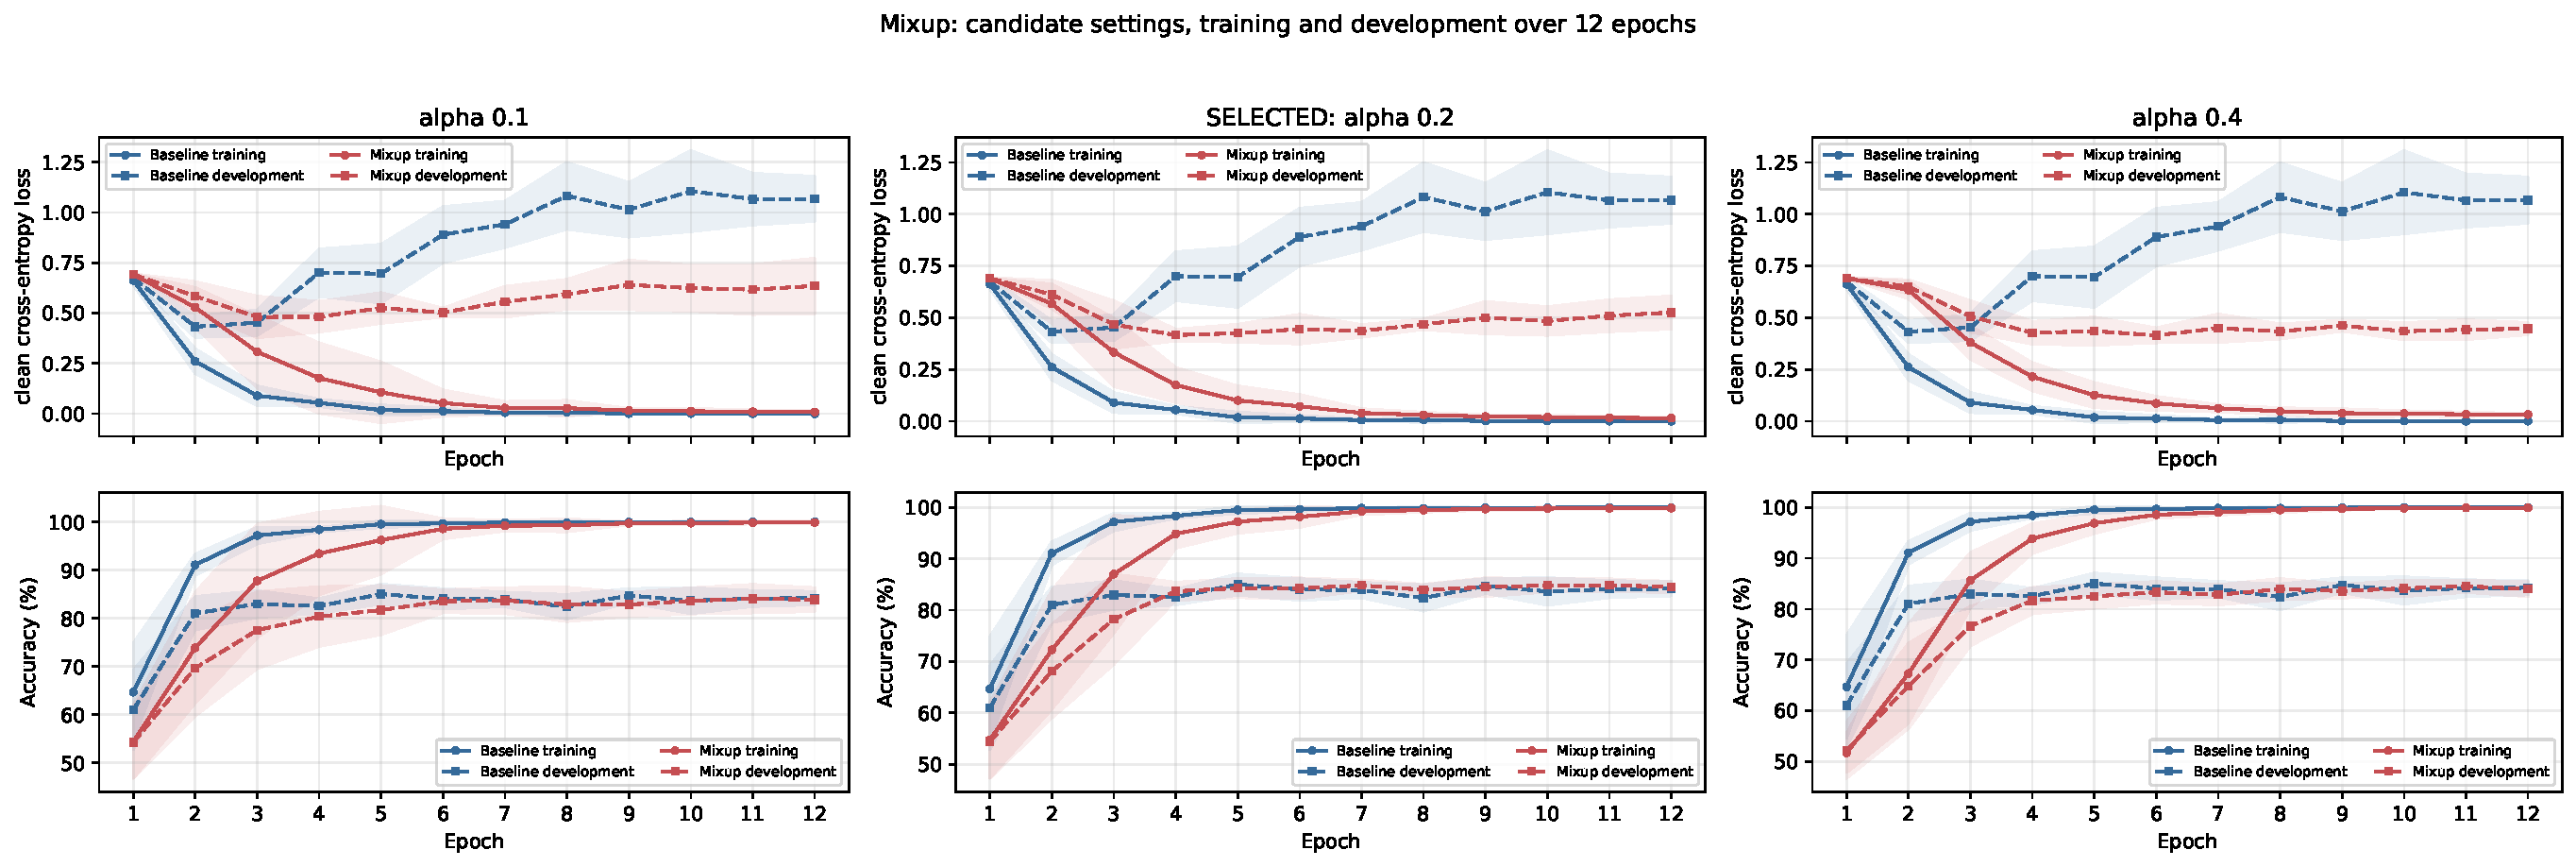
\includegraphics[width=0.96\textwidth]{curves_mixup.pdf}
\caption{Loss and accuracy over 12 epochs for the three Mixup strengths. Lines show seven-seed means; shading shows $\pm1$ standard deviation. The selected value is marked.}
\label{fig:curve-mixup}
\end{figure*}
}{}
}{}

\subsection{R-Drop}
R-Drop makes two forward passes with independent dropout masks and penalizes differences between their output distributions using symmetric KL divergence \cite{rdrop}. It can make predictions more stable, but larger penalties require more computation and may constrain learning too much. We compare $\lambda\in\{0.1,0.5,1.0\}$.
Figure~\ref{fig:curve-rdrop} compares the three R-Drop strengths with the baseline.
\IfFileExists{selection_results.tex}{%
\IfFileExists{curves_rdrop.pdf}{%
\begin{figure*}[tp]
\centering
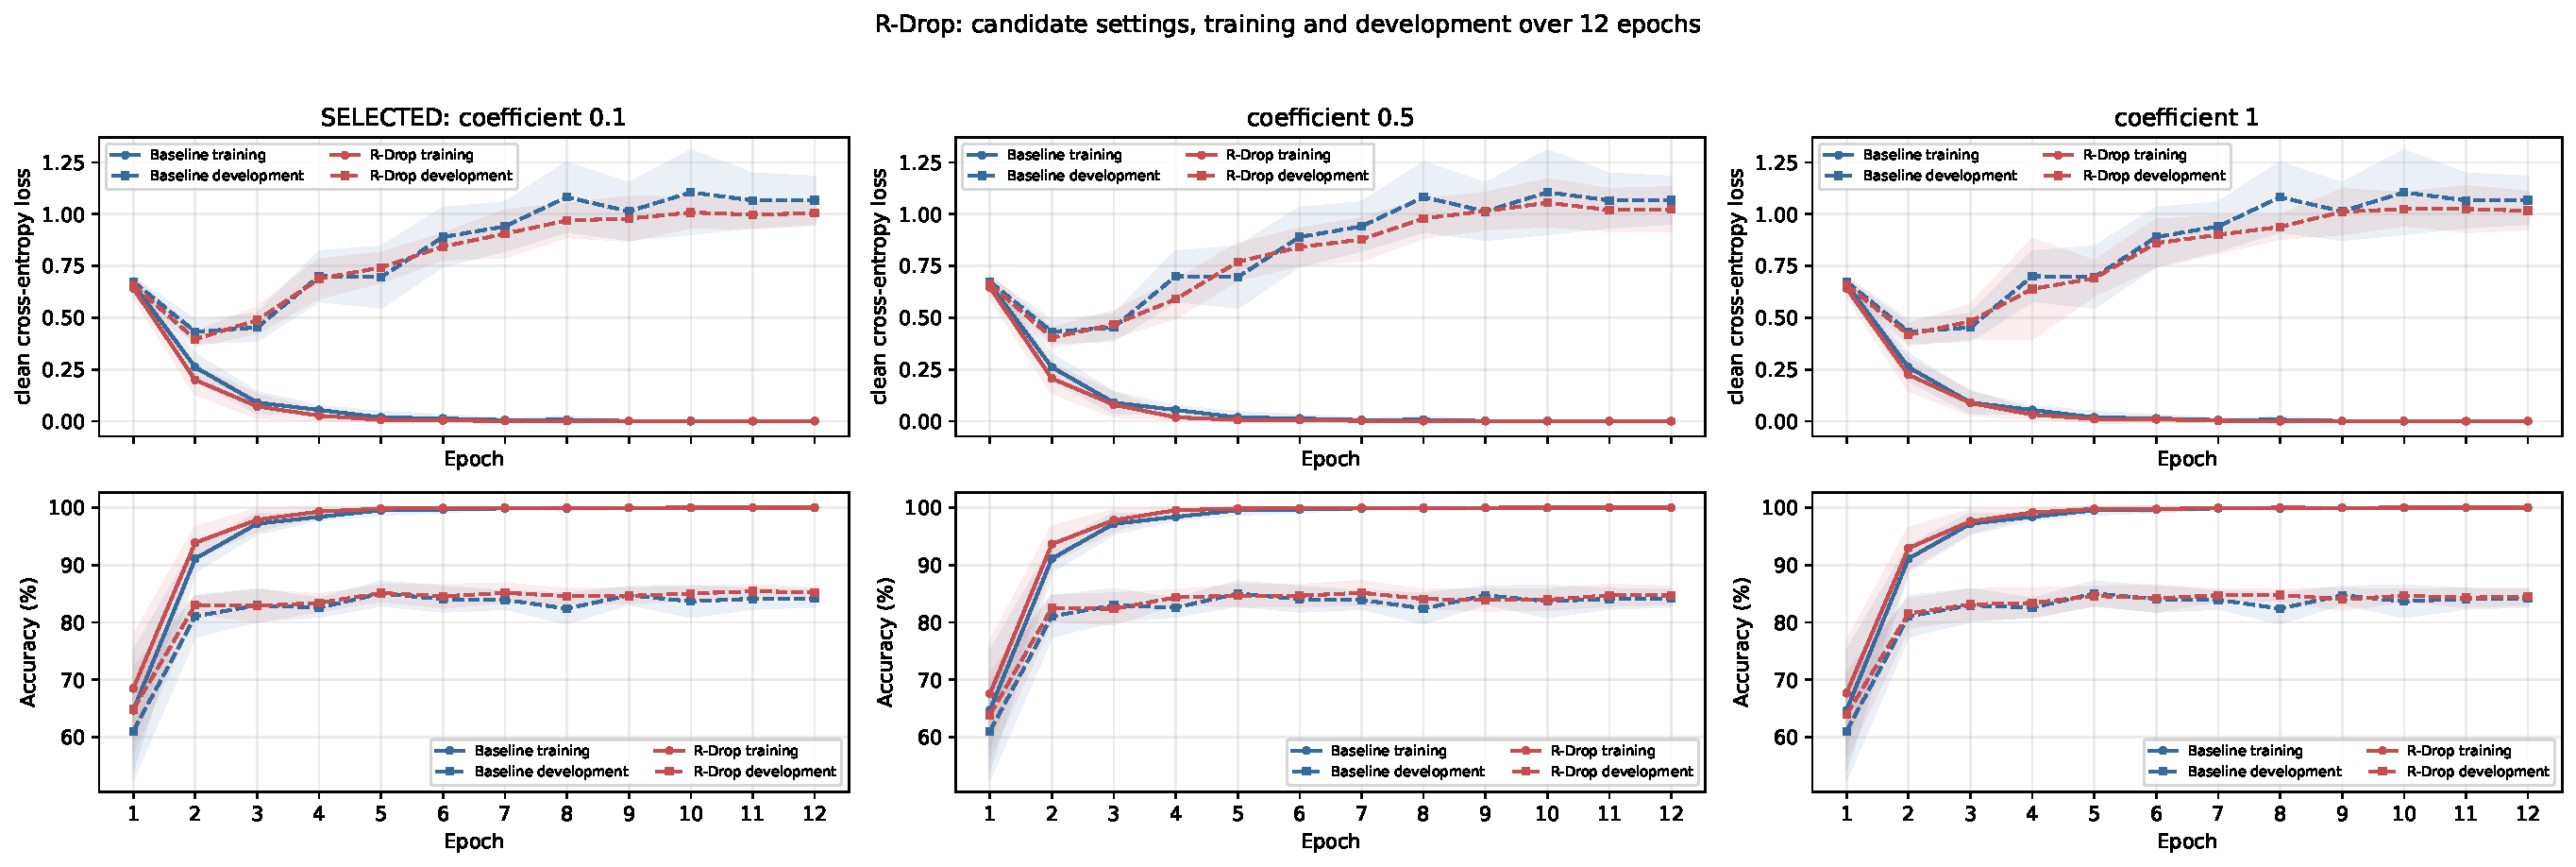
\includegraphics[width=0.96\textwidth]{curves_rdrop.pdf}
\caption{Loss and accuracy over 12 epochs for the three R-Drop coefficients. Lines show seven-seed means; shading shows $\pm1$ standard deviation. The selected value is marked.}
\label{fig:curve-rdrop}
\end{figure*}
}{}
}{}

\subsection{NEFTune}
NEFTune adds uniform noise to token embeddings during training \cite{neftune}. The noise scale is $\alpha/\sqrt{Ld}$, where $L$ is the number of unpadded tokens and $d$ is the embedding size; padding tokens are unchanged. Moderate noise may make representations more robust, while too much can obscure token information and hinder learning. We compare $\alpha\in\{5,10,15\}$ and evaluate on clean inputs.
Figure~\ref{fig:curve-neftune} compares the three noise scales with the baseline.
\IfFileExists{selection_results.tex}{%
\IfFileExists{curves_neftune.pdf}{%
\begin{figure*}[tp]
\centering
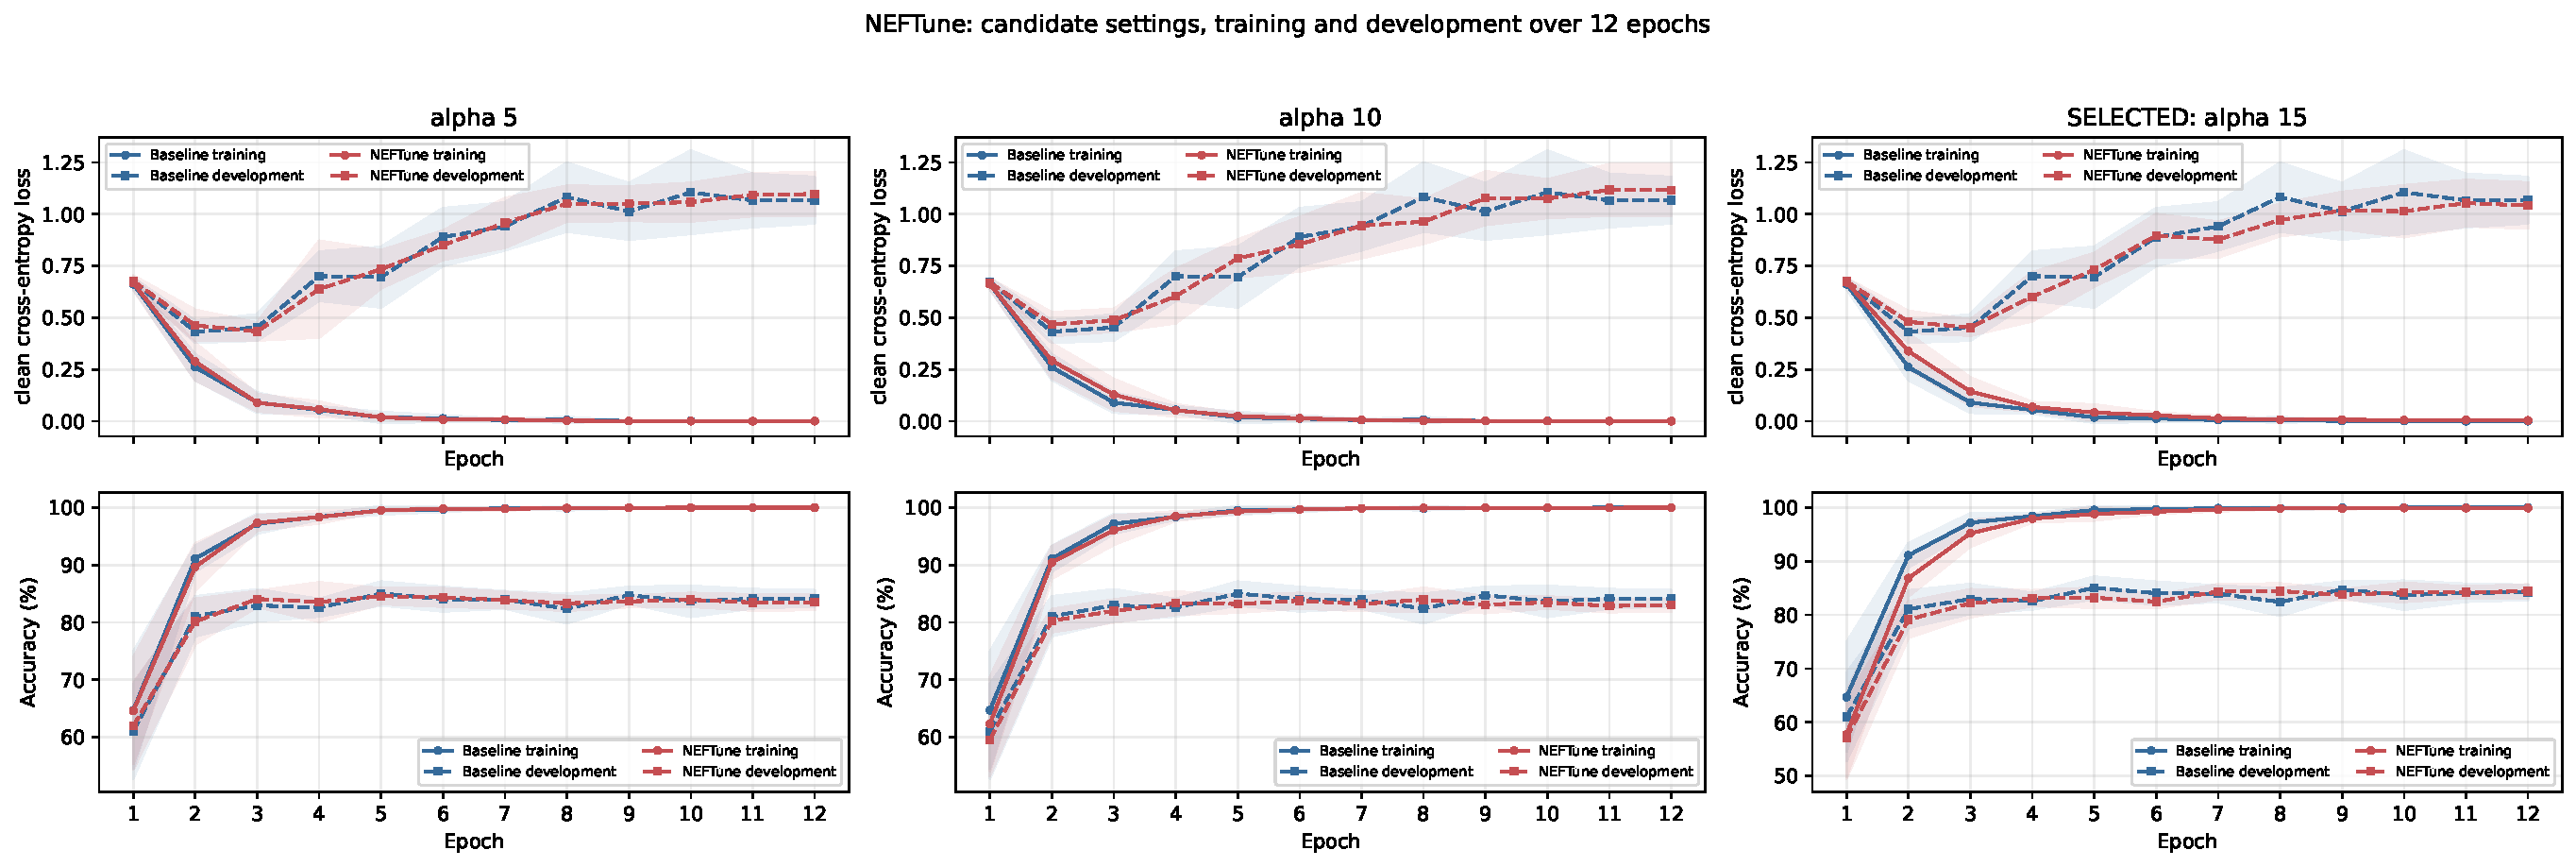
\includegraphics[width=0.96\textwidth]{curves_neftune.pdf}
\caption{Loss and accuracy over 12 epochs for the three NEFTune scales. Lines show seven-seed means; shading shows $\pm1$ standard deviation. The selected scale is marked.}
\label{fig:curve-neftune}
\end{figure*}
}{}
}{}

\subsection{Layer-Wise Learning-Rate Decay}
LLRD gives lower encoder layers smaller learning rates than upper layers, helping preserve pretrained representations while the model adapts to RTE \cite{ulmfit}. For layer $\ell$ in an $L$-layer encoder, $\eta_\ell=\eta\delta^{L-1-\ell}$. Embeddings receive one more decay step; the classifier uses the base rate $\eta$. Values of $\delta$ closer to one make layer rates more alike; smaller values reduce updates to lower layers and may limit their adaptation. We compare $\delta\in\{0.8,0.9,0.95\}$ at a base learning rate of $3\times10^{-5}$.
Figure~\ref{fig:curve-llrd} compares the three decay factors with the baseline.
\IfFileExists{selection_results.tex}{%
\IfFileExists{curves_llrd.pdf}{%
\begin{figure*}[tp]
\centering
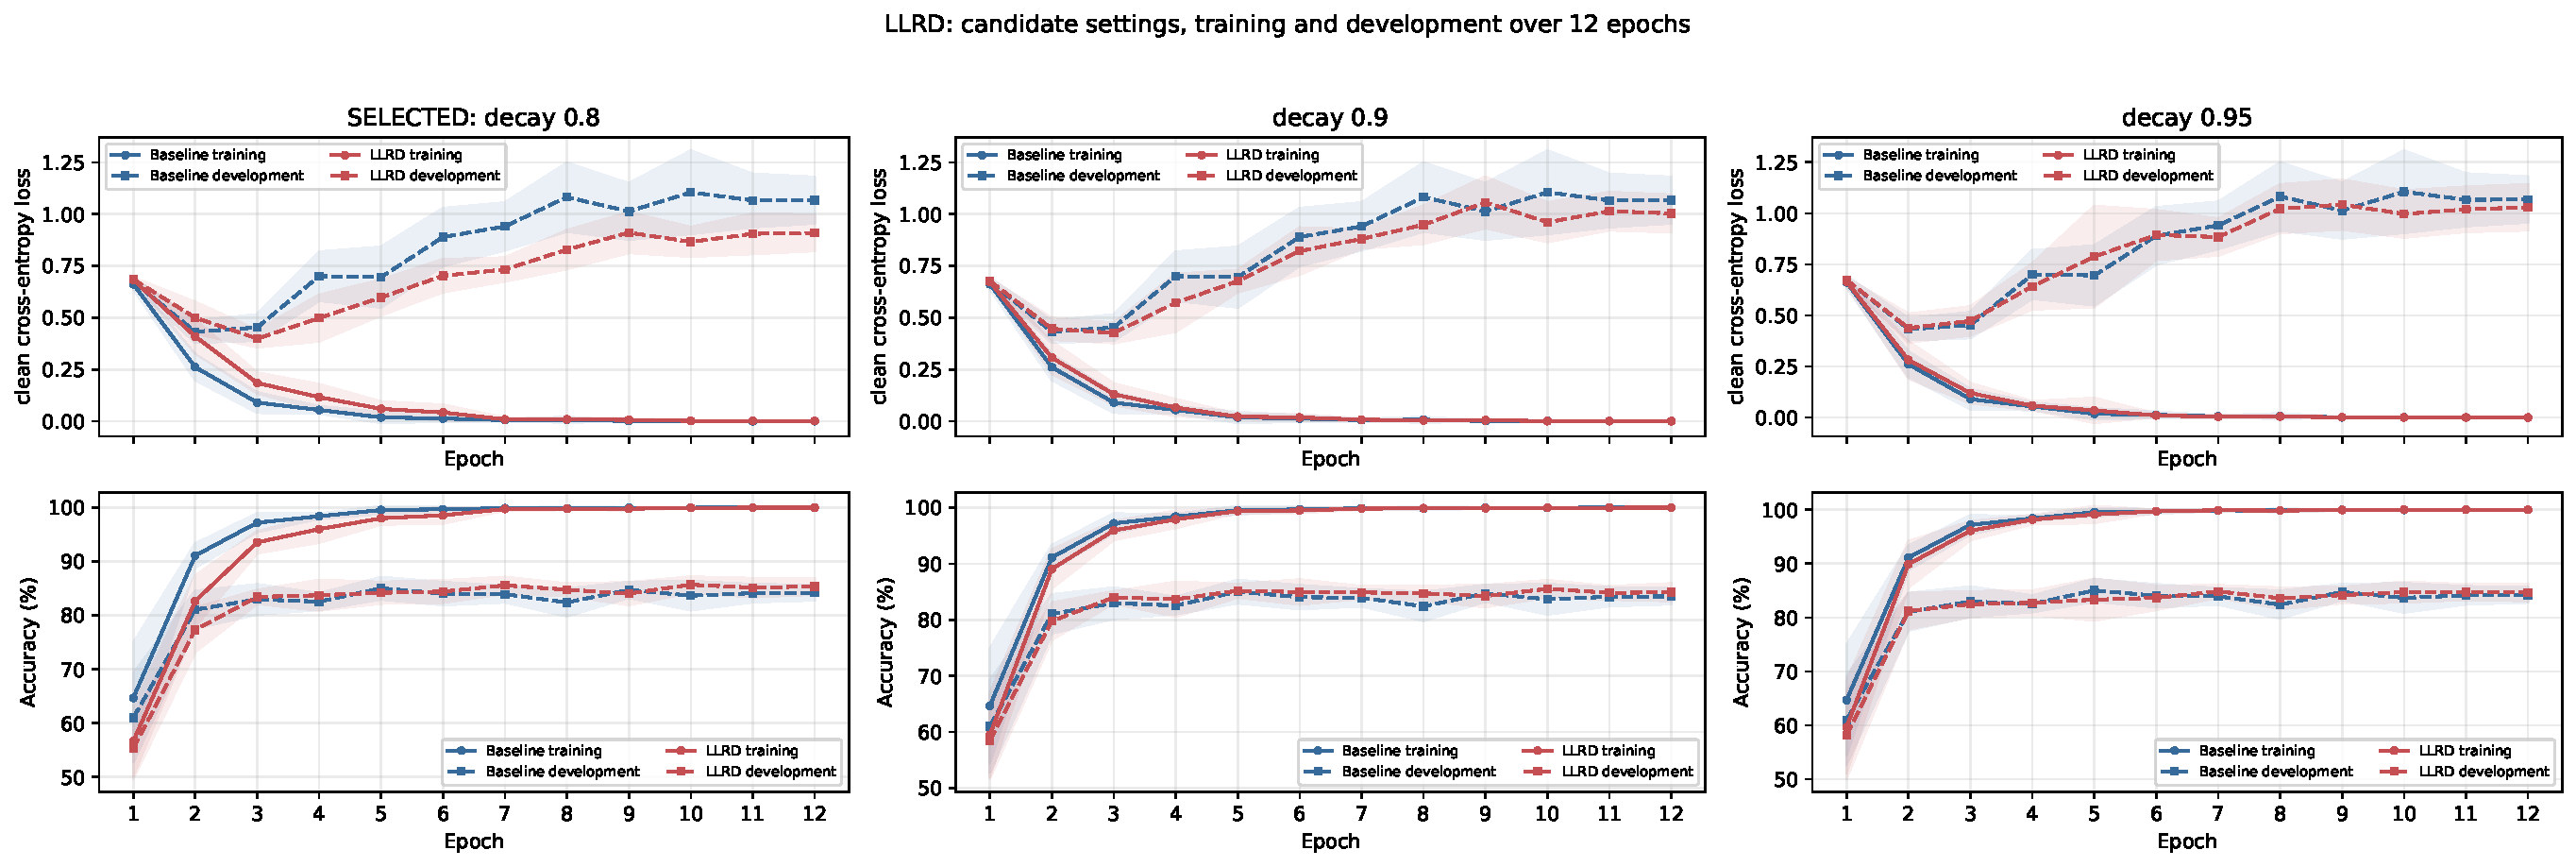
\includegraphics[width=0.96\textwidth]{curves_llrd.pdf}
\caption{Loss and accuracy over 12 epochs for the three LLRD decay factors. Lines show seven-seed means; shading shows $\pm1$ standard deviation. The selected decay is marked.}
\label{fig:curve-llrd}
\end{figure*}
}{}
}{}

\subsection{Optimized Combination}
The Optimized Combination uses only methods that pass the seven-seed baseline rule. We exclude a method if its mean paired gain is not positive or if fewer than four seeds beat the baseline. We combine the selected settings of the remaining methods and train for 12 epochs on all seven seeds. The selection table lists every include/exclude decision.
\IfFileExists{selection_results.tex}{%
\IfFileExists{curves_optimized_combination.pdf}{%
\begin{figure*}[tp]
\centering
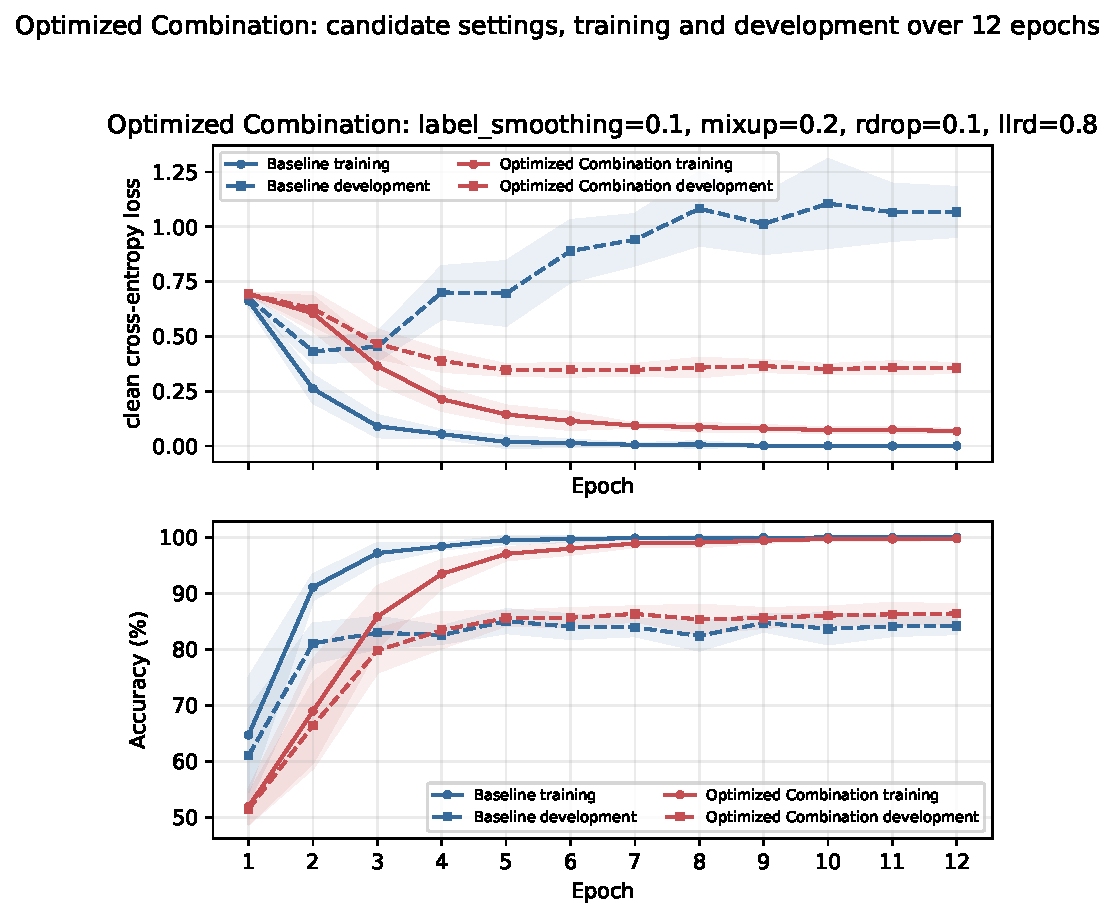
\includegraphics[width=0.82\textwidth]{curves_optimized_combination.pdf}
\caption{Loss and accuracy over 12 epochs for the Optimized Combination. Lines show seven-seed means; shading shows $\pm1$ standard deviation.}
\label{fig:curve-optimized-combination}
\end{figure*}
}{}
}{}

Figure~\ref{fig:pipeline} shows the training flow. Blue boxes mark techniques included in the Optimized Combination and the dropout forward pass used by selected R-Drop; gray boxes mark excluded candidates. Other process boxes are white. The diagram omits parameter values.

\begin{center}
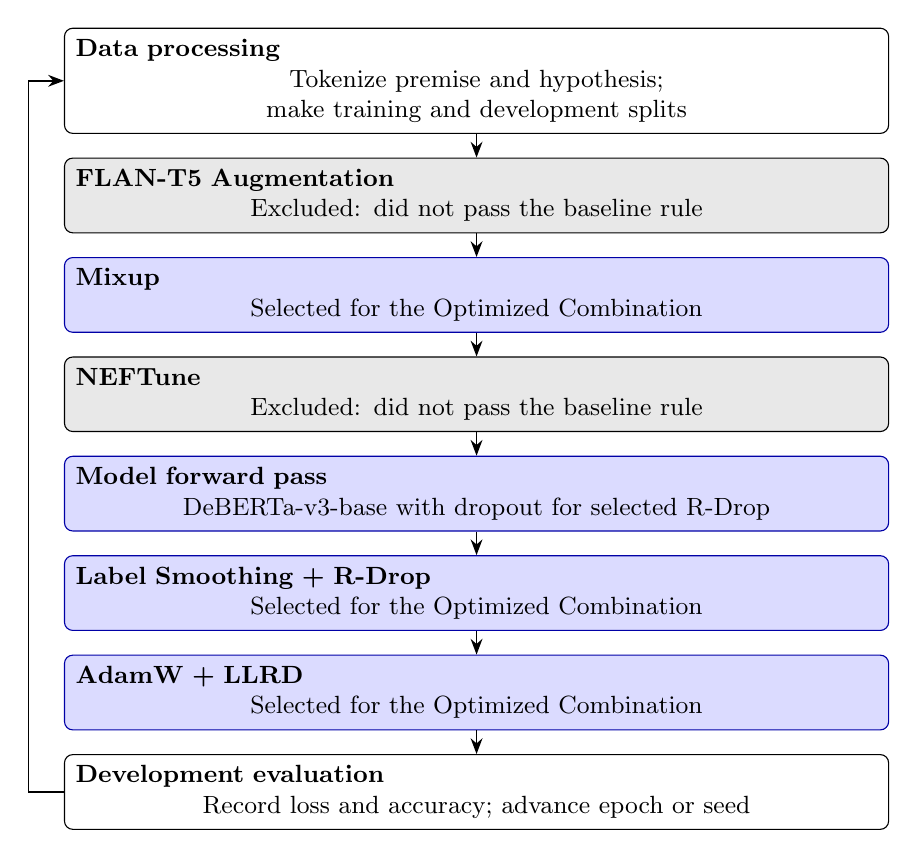
\begin{tikzpicture}[
	node distance=3mm,
	stage/.style={draw=black, rounded corners=3pt, align=center,
		text width=.84\columnwidth, minimum height=8mm, inner sep=4pt,
		font=\small, fill=white},
	selected/.style={stage, draw=blue!65!black, fill=blue!14},
	excluded/.style={stage, draw=black, fill=gray!18},
	flow/.style={-{Stealth[length=2mm]}, line width=.6pt}
]
\node[stage] (data) {\textbf{Data processing}\newline Tokenize premise and hypothesis; make training and development splits};
\node[excluded, below=of data] (augmentation) {\textbf{FLAN-T5 Augmentation}\newline Excluded: did not pass the baseline rule};
\node[selected, below=of augmentation] (mixup) {\textbf{Mixup}\newline Selected for the Optimized Combination};
\node[excluded, below=of mixup] (neftune) {\textbf{NEFTune}\newline Excluded: did not pass the baseline rule};
\node[selected, below=of neftune] (encoder) {\textbf{Model forward pass}\newline DeBERTa-v3-base with dropout for selected R-Drop};
\node[selected, below=of encoder] (objective) {\textbf{Label Smoothing + R-Drop}\newline Selected for the Optimized Combination};
\node[selected, below=of objective] (optimizer) {\textbf{AdamW + LLRD}\newline Selected for the Optimized Combination};
\node[stage, below=of optimizer] (feedback) {\textbf{Development evaluation}\newline Record loss and accuracy; advance epoch or seed};
\draw[flow] (data.south) -- (augmentation.north);
\draw[flow] (augmentation.south) -- (mixup.north);
\draw[flow] (mixup.south) -- (neftune.north);
\draw[flow] (neftune.south) -- (encoder.north);
\draw[flow] (encoder.south) -- (objective.north);
\draw[flow] (objective.south) -- (optimizer.north);
\draw[flow] (optimizer.south) -- (feedback.north);
\draw[flow] (feedback.west) -- ++(-0.45,0) |- (data.west);
\end{tikzpicture}
\captionof{figure}{Inline training pipeline for the Optimized Combination. Blue marks selected techniques and the dropout forward pass used by R-Drop; gray marks excluded candidates. The loop covers 12 epochs for each seed.}
\label{fig:pipeline}
\end{center}

\section{Results and Hyperparameter Selection}
All curves and tables summarize 12-epoch runs over the same seven seeds. We compare candidates by mean final development accuracy, using development loss to break ties. Because the development set is also used for selection, it is not an independent test set. The tables below are generated from the saved run metrics.

\IfFileExists{selection_results.tex}{\begin{table*}[tp]
\centering\scriptsize\setlength{\tabcolsep}{3pt}
\caption{Candidate settings after 12 epochs and 7 seeds. Include a method only if its mean paired gain is positive and a majority of seeds beat baseline.}
\label{tab:selected-hyperparameters}
\begin{tabular}{p{0.16\textwidth}p{0.13\textwidth}p{0.20\textwidth}rrrp{0.13\textwidth}}
\toprule
Method & Candidates & Selected & Dev acc. (\%) & Gain (pp) & Dev loss & Decision \\
\midrule
Baseline & -- & -- & 84.19 & -- & 1.068 & -- \\
Filtered augmentation & 0.25, 0.5, 1 & ratio=0.5 & 84.00 & -0.19 & 1.171 & 3/7; exclude \\
Label smoothing & 0.05, 0.1, 0.15 & epsilon=0.1 & 84.61 & +0.42 & 0.454 & 4/7; include \\
Mixup & 0.1, 0.2, 0.4 & alpha=0.2 & 84.53 & +0.34 & 0.525 & 4/7; include \\
NEFTune & 5, 10, 15 & alpha=15 & 84.38 & +0.19 & 1.042 & 3/7; exclude \\
R-Drop & 0.1, 0.5, 1 & coefficient=0.1 & 85.22 & +1.03 & 1.005 & 5/7; include \\
LLRD & 0.8, 0.9, 0.95 & decay=0.8 & 85.37 & +1.18 & 0.910 & 5/7; include \\
Optimized Combination & Label smoothing, Mixup, R-Drop, LLRD & smoothing=0.1, Mixup=0.2, R-Drop=0.1, LLRD=0.8 & 86.40 & +2.22 & 0.356 & 6/7 \\
\bottomrule
\end{tabular}
\end{table*}
\begin{table*}[tp]
\centering\scriptsize\setlength{\tabcolsep}{3pt}
\caption{Final development accuracy (\%) for all 7 seeds after 12 epochs, ranked by Optimized Combination gain. Every seed remains in the analysis.}
\label{tab:selected-seeds}
\begin{tabular}{rrrrrrrrrrr}
\toprule
Rank & Seed & Baseline & Aug. & Smooth. & Mixup & R-Drop & NEFTune & LLRD & Optimized & Gain (pp) \\
\midrule
1 & 456 & 82.35 & 82.89 & 83.69 & 84.49 & 84.76 & 85.29 & 87.43 & 86.90 & +4.55 \\
2 & 123 & 83.69 & 83.42 & 84.22 & 85.56 & 85.83 & 84.22 & 85.56 & 87.70 & +4.01 \\
3 & 789 & 83.42 & 84.76 & 82.09 & 83.16 & 85.56 & 83.42 & 83.69 & 86.10 & +2.67 \\
4 & 1801564980 & 85.29 & 84.22 & 85.29 & 86.10 & 84.22 & 84.76 & 85.29 & 87.43 & +2.14 \\
5 & 201765793 & 86.63 & 85.56 & 83.42 & 83.69 & 84.49 & 85.03 & 86.90 & 87.97 & +1.34 \\
6 & 1011 & 83.69 & 84.22 & 87.17 & 83.69 & 85.83 & 85.83 & 85.29 & 84.76 & +1.07 \\
7 & 1323889826 & 84.22 & 82.89 & 86.36 & 85.03 & 85.83 & 82.09 & 83.42 & 83.96 & -0.27 \\
\bottomrule
\end{tabular}
\end{table*}
}{Candidate-selection and per-seed tables will be populated from the completed seven-seed runs.}
\IfFileExists{evaluation_matrix.tex}{\begin{table*}[tp]
\centering\small\setlength{\tabcolsep}{4pt}
\caption{Final-epoch metrics after 12 epochs, mean $\pm$ sample SD over seven seeds. Training loss is clean evaluation-mode loss. Augmentation training metrics use the augmented training split.}
\label{tab:evaluation-matrix}
\begin{tabular}{p{0.27\textwidth}rrrr}
\toprule
Method & Train accuracy (\%) & Train loss & Validation accuracy (\%) & Validation loss \\
\midrule
Baseline & $99.99 \pm 0.02$ & $0.00 \pm 0.00$ & $84.19 \pm 1.39$ & $1.07 \pm 0.11$ \\
Filtered augmentation (augmentation=0.5) & $99.99 \pm 0.02$ & $0.00 \pm 0.00$ & $84.00 \pm 0.99$ & $1.17 \pm 0.08$ \\
Label smoothing (epsilon=0.1) & $100.00 \pm 0.00$ & $0.04 \pm 0.00$ & $84.61 \pm 1.77$ & $0.45 \pm 0.05$ \\
Mixup (mixup=0.2) & $99.88 \pm 0.16$ & $0.01 \pm 0.00$ & $84.53 \pm 1.09$ & $0.53 \pm 0.08$ \\
NEFTune (neftune=15) & $99.89 \pm 0.08$ & $0.00 \pm 0.00$ & $84.38 \pm 1.27$ & $1.04 \pm 0.11$ \\
R-Drop (rdrop=0.1) & $99.99 \pm 0.02$ & $0.00 \pm 0.00$ & $85.22 \pm 0.70$ & $1.00 \pm 0.06$ \\
LLRD (llrd=0.8) & $99.98 \pm 0.03$ & $0.00 \pm 0.00$ & $85.37 \pm 1.49$ & $0.91 \pm 0.09$ \\
Optimized Combination & $99.77 \pm 0.17$ & $0.07 \pm 0.01$ & $86.40 \pm 1.54$ & $0.36 \pm 0.02$ \\
\bottomrule
\end{tabular}
\end{table*}
}{The training and validation metric matrix will be added from the completed runs.}

\subsection{Internal Held-Out Test (Exploratory)}
After selecting settings on development data, we evaluate the baseline and Optimized Combination on the 374-example internal holdout. Earlier studies examined this split, so it is held out from these training runs but is not an untouched test set. The table reports per-seed accuracy and paired gains.
\IfFileExists{heldout_results.tex}{\begin{table*}[tp]
\centering\small\setlength{\tabcolsep}{4pt}
\caption{Internal holdout accuracy for seven matched seeds after 12 epochs. The 374-example split was examined in prior studies; results are exploratory, not an independent test.}
\label{tab:heldout-accuracy}
\begin{tabular}{lrrr}
\toprule
Seed & Baseline accuracy (\%) & Optimized Combination (\%) & Gain (pp) \\
\midrule
123 & 77.27 & 85.03 & +7.75 \\
456 & 79.41 & 83.69 & +4.28 \\
789 & 77.01 & 84.49 & +7.49 \\
1011 & 83.16 & 85.03 & +1.87 \\
201765793 & 83.42 & 84.76 & +1.34 \\
1801564980 & 81.82 & 85.83 & +4.01 \\
1323889826 & 80.21 & 83.69 & +3.48 \\
\midrule
Mean $\pm$ SD & 80.33 $\pm$ 2.61 & 84.64 $\pm$ 0.77 & +4.32 \\
\bottomrule
\end{tabular}
\end{table*}
}{The internal holdout comparison will be added after the final evaluation runs complete.}

Read training and development curves together. Lower training loss alone may mean the model is memorizing; a growing gap between training and development loss may signal overfitting. We select settings by the stated development rule, not by how smooth a curve looks. The Optimized Combination tests the selected methods together, so it cannot show each method's separate effect.

\section{Conclusion}
This report covers full-fine-tuning runs with 12 epochs and seven matched seeds. We compare every selected technique with the same baseline and include only methods that pass the four-of-seven rule. On the previously examined internal holdout, the Optimized Combination averaged 84.64\% accuracy, compared with 80.33\% for baseline; its paired gain was 4.32 points, and all seven seeds improved. These holdout results are exploratory because the split was examined in earlier studies. The Optimized Combination does not isolate each method's effect. A follow-up should evaluate the fixed settings on new labeled data that were not used for selection.

\begin{thebibliography}{11}
\bibitem[He et~al.(2021)]{deberta} He et al. (2021). DeBERTaV3. \url{https://arxiv.org/abs/2111.09543}.
\bibitem[Wang et~al.(2018)]{glue} Wang et al. (2018). GLUE. \url{https://arxiv.org/abs/1804.07461}.
\bibitem[Liang et~al.(2021)]{rdrop} Liang et al. (2021). R-Drop. \url{https://arxiv.org/abs/2106.14448}.
\bibitem[Chung et~al.(2022)]{flan} Chung et al. (2022). Scaling Instruction-Finetuned Language Models. \url{https://arxiv.org/abs/2210.11416}.
\bibitem[M\"uller et~al.(2019)]{smoothing} M\"uller et al. (2019). When Does Label Smoothing Help? \url{https://arxiv.org/abs/1906.02629}.
\bibitem[Zhang et~al.(2018)]{mixup} Zhang et al. (2018). mixup: Beyond Empirical Risk Minimization. \url{https://arxiv.org/abs/1710.09412}.
\bibitem[Jain et~al.(2023)]{neftune} Jain et al. (2023). NEFTune: Noisy Embeddings Improve Instruction Finetuning. \url{https://arxiv.org/abs/2310.05914}.
\bibitem[Howard and Ruder(2018)]{ulmfit} Howard and Ruder (2018). Universal Language Model Fine-tuning for Text Classification. ACL. \url{https://aclanthology.org/P18-1031/}.
\bibitem[Kobyzev et~al.(2023)]{kobyzev2023} Kobyzev, I., Jafari, A., Rezagholizadeh, M., Li, T., Do-Omri, A., Lu, P., Poupart, P., and Ghodsi, A. 2023. Do We Need Label Regularization to Fine-Tune Pre-trained Language Models? In Proceedings of EACL 2023, pages 166--177. \url{https://aclanthology.org/2023.eacl-main.13/}.
\bibitem[Somayajula et~al.(2024)]{somayajula2024} Somayajula, S. A., Liang, Y., Zhang, L., Singh, A., and Xie, P. 2024. Generalizable and Stable Finetuning of Pretrained Language Models on Low-Resource Texts. In Proceedings of NAACL-HLT 2024, pages 4936--4953. \url{https://aclanthology.org/2024.naacl-long.277/}.
\bibitem[Juki\'c and \v{S}najder(2025)]{jukic2025} Juki\'c, J., and \v{S}najder, J. 2025. From Robustness to Improved Generalization and Calibration in Pre-trained Language Models. Transactions of the Association for Computational Linguistics, 13:264--280. \url{https://aclanthology.org/2025.tacl-1.13/}.
\end{thebibliography}

\end{document}


